\newpage
\subsection{UC1 - Creazione ambiente}
\label{subsec:uc1}

%TODO: Add correct image
% Se uno use case esce dalla post allora non mettiamo in scenario secondario ma in estensione
% se invece la post rimane la stessa non è estensione.

\begin{figure}[h]
    \centering
    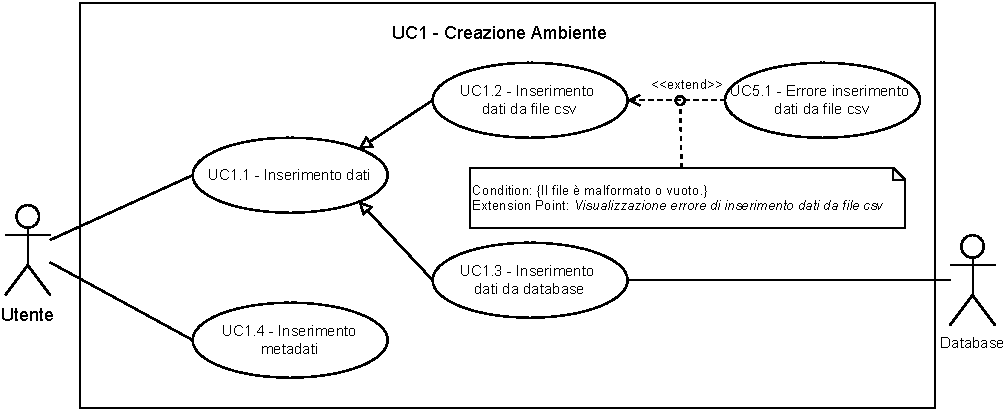
\includegraphics[width=0.6\textwidth]{componenti/casi-duso/diagrammi/UC1.pdf}
    \caption{Diagramma rappresentante UC1}
    \label{fig:UC1}
\end{figure}


\begin{itemize}
    \item \textbf{Descrizione}: L'utente prepara l'applicativo HDviz alla rappresentazione
                                grafica dei dati importando l'opportuno dataset e assegna, 
                                se non già definiti, dei metadati 
                                che descrivono il tipo del dato di ogni colonna.
	
    \item \textbf{Attore primario}: Utente;
    \item \textbf{Attore secondario}: Database;
    
    
    \item \textbf{Precondizione}:   L'utente decide di caricare i dati.

    \item \textbf{Postcondizione}:  Viene caricato un dataset. 
    
                                    Ogni colonna del dataset ha associato
                                    un metatag che indica la tipologia del dato.

	\item \textbf{Scenario principale}:
		\begin{enumerate}
			\item L'utente seleziona l'opzione di aggiunta dei dati.
            \item L'utente seleziona la fonte dei dati da importare e li importa.
            \item Il dataset caricato è corretto e provvisto di validi metatag.
        \end{enumerate}
   
    \item \textbf{Scenario alternativo}:
		\begin{enumerate}
            \item Il dataset caricato presenta metatag non validi o ne è sprovvisto:
            \begin{enumerate}
                \item L'utente inserisce manualmente i metatag (UC1.4).
            \end{enumerate}
        \end{enumerate}

    \item \textbf{Generalizzazioni}:
    \begin{enumerate}
        \item Inserimento dati da file csv.
        \item Inserimento dati da database.
    \end{enumerate}
\end{itemize}


\subsection{UC1.1 - Inserimento dati}
\label{ssub:UC1.1}
\begin{itemize}
    \item \textbf{Descrizione}: L'utente decide di impostare l'ambiente creando un dataset i cui 
                                dati vengono caricati da file csv oppure da database al quale l'utente ha accesso.

    \item \textbf{Attore primario}: Utente.
    \item \textbf{Attore secondario}: Database;
    
    \item \textbf{Precondizione}:   L'utente decide di caricare i dati.

    \item \textbf{Postcondizione}:  Viene caricato un dataset non vuoto dalla fonte scelta dall'utente. 

	\item \textbf{Scenario principale}:
		\begin{enumerate}
			\item L'utente seleziona l'opzione di aggiunta dei dati:
            \begin{enumerate}
                \item L'utente sceglie di importare i dati da file (UC1.2)
                \item L'utente seleziona di importare i dati da database (UC1.3)
            \end{enumerate}
        \end{enumerate}

        \item \textbf{Generalizzazioni}:
        \begin{enumerate}
            \item Inserimento dati da file csv. (UC1.2)
            \item Inserimento dati da database. (UC1.3)
        \end{enumerate}
\end{itemize}


\begin{figure}[h]
    \centering
    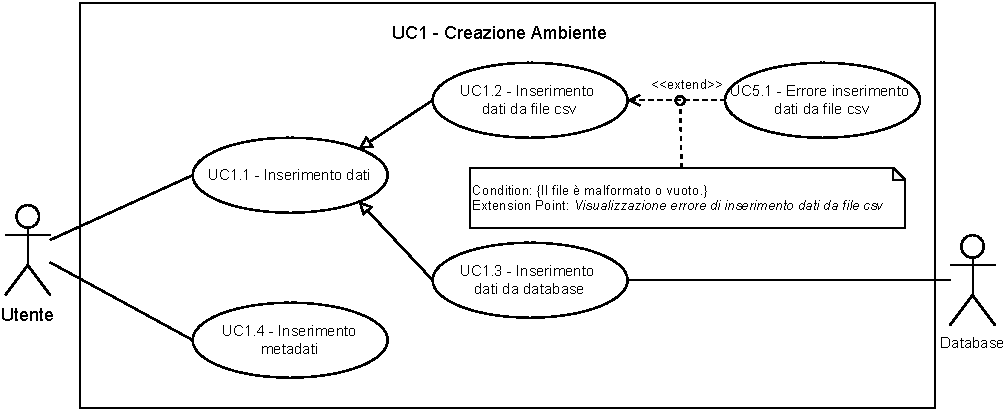
\includegraphics[width=0.8\textwidth]{componenti/casi-duso/diagrammi/UC1.pdf}
    \caption{Diagramma rappresentante UC1}
    \label{fig:UC1}
\end{figure}


\subsubsection{UC1.2 - Inserimento dati da file csv}
\label{ssub:UC1.1.1}
\begin{itemize}
    \item \textbf{Descrizione}: L'utente importa un dataset non vuoto da un file csv del suo dispostivo.

    \item \textbf{Attore primario}: Utente.
    
    \item \textbf{Precondizione}:   L'utente selezione l'opzione di caricare i dati da un file .csv .
    \item \textbf{Postcondizione}:  Viene caricato un dataset. 

	\item \textbf{Scenario principale}:
		\begin{enumerate}
			\item L'utente seleziona l'opzione di aggiunta dei dati mediante file.
			\item L'utente seleziona file di dati valido da importare.
        \end{enumerate}
     
    \item \textbf{Estensioni}
    \begin{enumerate}
    
        \item Se l'utente importa un file non valido oppure vuoto:
        \begin{enumerate}
            \item La creazione del dataset falllsice
            \item Viene visualizzato il messaggio di errore. (UC5.1.1)
        \end{enumerate}
    \end{enumerate}
\end{itemize}

\newpage
\begin{figure}[h]
    \centering
    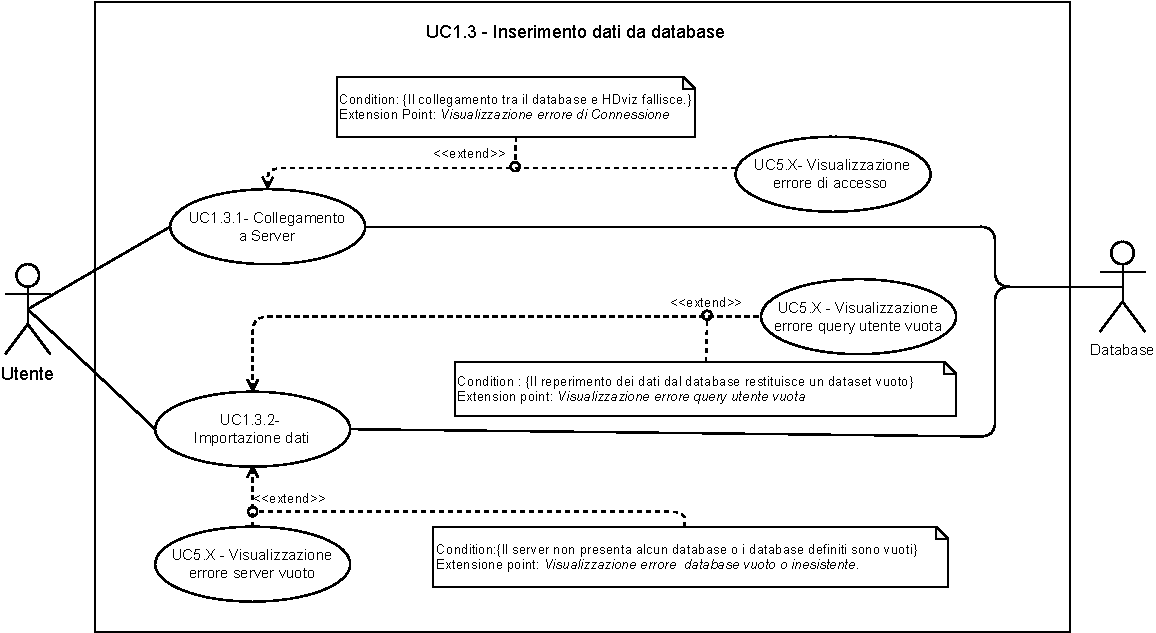
\includegraphics[width=0.9\textwidth]{componenti/casi-duso/diagrammi/UC1.3.pdf}
    \caption{Diagramma rappresentante UC1.3}
    \label{fig:UC1.3}
\end{figure}


\subsection{UC1.3 - Inserimento dati da database}
\label{ssub:UC1.3}
\begin{itemize}
    \item \textbf{Descrizione}: L'utente si connette ad un database di cui dispone accesso e 
                                crea un dataset non vuoto dal risultato di una ricerca delle tabelle che gli interessano
                                visualizzare successivamente in HDviz.
    \item \textbf{Attore primario}: Utente.
    
    \item \textbf{Attore secondario}: Database.
    
    \item \textbf{Precondizione}:   L'utente decide di caricare i dati ed ha accesso ad un database.

    \item \textbf{Postcondizione}:  Viene caricato un dataset dal database.

	\item \textbf{Scenario principale}:
		\begin{enumerate}
			\item L'utente effettua la connessione con un database da lui fornito.
			\item L'utente importa i dati secondo la modalità che lui sceglie.
        \end{enumerate}

    \item \textbf{Estensioni}:
    \begin{enumerate}
        \item Se l'apertura della connessione con il database fallisce.
        \begin{enumerate}
            \item L'inserimento dei dati viene interrotto.
            \item Viene visualizzato un messaggio di errore (UC5.2).
        \end{enumerate}

        \item Se il server al quale si è connessi non ha database o tutti sono vuoti.
        \begin{enumerate}
            \item L'inserimento dei dati viene interrotto.
            \item Viene visualizzato un messaggio di errore (UC5.3).
        \end{enumerate}

        \item Se la query utente è vuota o il risultano non ha almeno due dimensioni:
        \begin{enumerate}
            %TODO: Qui potrebbe continuare il flow normale basta fargli rimettere la cosa.
            \item L'inserimento dei dati viene interrotto.
            \item Viene visualizzato un messaggio di errore (UC5.4).
        \end{enumerate}
    \end{enumerate}
\end{itemize}


\newpage
\begin{figure}[h]
    \centering
    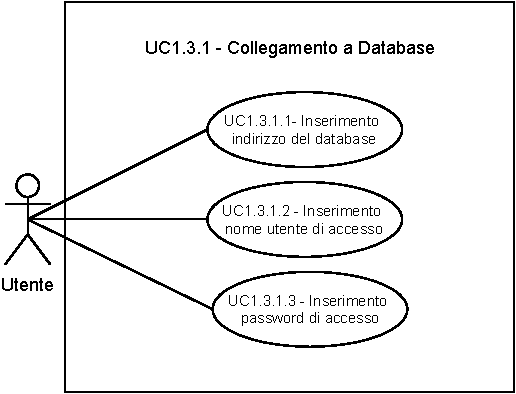
\includegraphics[width=0.6\textwidth]{componenti/casi-duso/diagrammi/UC1.3.1.pdf}
    \caption{Diagramma rappresentante UC1.3.1}
    \label{fig:UC1.3}
\end{figure}


\subsection{UC1.3.1 - Collegamento a Server}
\label{ssub:UC1.3}
\begin{itemize}
    \item \textbf{Descrizione}: L'utente apre una connessione con un server di dati del quale 
                                dispone le credenziali di accesso. 

    \item \textbf{Attore primario}: Utente.
    \item \textbf{Attore secondario}: Database.
    
    \item \textbf{Precondizione}:   L'utente decide di caricare i dati mediante un database.
    \item \textbf{Postcondizione}:  Viene aperta la connessione con un server di dati.

	\item \textbf{Scenario principale}:
		\begin{enumerate}
			\item L'utente immette i campi necessari per l'acceso: indirizzo, nome utente e password.
			\item HDviz si connette al server con i valori immessi dall'utente.
        \end{enumerate}
    \end{itemize}


\subsubsection{UC1.3.1.1 - Inserimento indirizzo}
\label{ssub:UC1.3}
\begin{itemize}
    \item \textbf{Descrizione}: L'utente inserisce l'indirizzo del server al quale vuole accedere.
    \item \textbf{Attore primario}: Utente.    
   
    \item \textbf{Precondizione}:   L'utente decide di caricare un dataset mediante un database.
    \item \textbf{Postcondizione}:  Viene inserito l'indirizzo del server di dati.
    
    \item \textbf{Scenario Principale}: L'utente inserisce l'indirizzo di connessione.

\end{itemize}


\subsubsection{UC1.3.1.2 - Inserimento nome utente}
\label{ssub:UC1.3}
\begin{itemize}
    \item \textbf{Descrizione}: L'utente inserisce il nome utente per accedere al server.
    \item \textbf{Attore primario}: Utente.
    
    \item \textbf{Precondizione}:   L'utente decide di caricare i dataset meidante un database.
    \item \textbf{Postcondizione}:  Viene inserito il nome utente per l'accessp al server di dati.

    \item \textbf{Scenario Principale}: L'utente inserisce il nome d'accesso.
\end{itemize}


\subsubsection{UC1.3.1.3 - Inserimento password}
\label{ssub:UC1.3}
\begin{itemize}
    \item \textbf{Descrizione}: L'utente inserisce la password per accedere al server.
    \item \textbf{Attore primario}: Utente.
    
    \item \textbf{Precondizione}:   L'utente decide di caricare i dataset meidante un database.
    \item \textbf{Postcondizione}:  Viene caricato un dataset dal database.

    \item \textbf{Scenario Principale}: L'utente inserisce la password d'accesso.

\end{itemize}


\subsection{UC1.3.2 - Importazione dati}
\label{subsec:UC1.3}
\begin{itemize}
    \item \textbf{Descrizione}: L'utente ottiene i dati che da inserire nel nuovo dataset da un database
                                del server con cui ha una connessione aperta al momento, mediante 
                                l'esecuzione di una query personalizzata che fornisce come file.

    \item \textbf{Attore primario}: Utente.
    
    \item \textbf{Attore secondario}: Database.
    
    \item \textbf{Precondizione}:   L'utente ha aperto una connessione con un server dati.
    \item \textbf{Postcondizione}:  Viene costruito il dataset dai dati reperiti dall'utente mediante un file di query.

	\item \textbf{Scenario principale}:
		\begin{enumerate}
			\item L'utente carica un file di query che viene eseguito sul server.
			\item Viene costruito il dataset dal risultato della ricerca.
        \end{enumerate}

    %TODO CApire dove diamine vanno messe le estensioni.
\end{itemize}






\subsection{UC1.4 - Inserimento metadati}
\label{ssub:UC1.2}
\begin{itemize}
    \item \textbf{Descrizione}: L'utente assegna ad ogni colonna del dataset importato,
                                in cui non è già correttamente definito,
                                dei metatag che ne descrivono le proprietà.


    \item \textbf{Attore primario}: Utente.
    
    \item \textbf{Precondizione}:   L'utente ha caricato un dataset e non tutti i suoi metadati sono validi o definiti.
    \item \textbf{Postcondizione}:  Il dataset caricato è provvisto di metadati validi. 

	\item \textbf{Scenario principale}:
		\begin{enumerate}
            \item L'utente assegna ad ogni colonna del dataset il tipo di dato che rappresenta (metatag) scegliendo tra:
                \begin{enumerate}
                    \item Nominale 
                    \item Ordinale 
                    \item Intervallo
                    \item Rapporto
                \end{enumerate}
        \end{enumerate}

\end{itemize}

